\documentclass[a4paper,12pt]{article}
\usepackage[utf8]{inputenc}
\usepackage[german]{babel}
\usepackage{amsmath}
\usepackage{amssymb}
\usepackage{amsthm}
\usepackage{geometry}
\usepackage{graphicx}
\usepackage[hidelinks]{hyperref}
\usepackage{listings}
\usepackage{xcolor}
\usepackage{enumitem}
\usepackage{booktabs}
\usepackage{array}
\usepackage{float}

\geometry{margin=2.5cm}

\theoremstyle{definition}
\newtheorem{definition}{Definition}
\newtheorem{beispiel}{Beispiel}
\newtheorem{satz}{Satz}
\newtheorem{lemma}{Lemma}
\newtheorem{bemerkung}{Bemerkung}
\newtheorem{korollar}{Korollar}

\setlist[itemize,1]{label=--}

\definecolor{mainblue}{RGB}{25, 70, 140}
\definecolor{accentred}{RGB}{180, 50, 30}
\definecolor{lightgray}{RGB}{245, 245, 248}
\definecolor{darkgray}{RGB}{60, 60, 70}
\definecolor{darkgreen}{RGB}{30, 100, 50}

\hypersetup{
    colorlinks=true,
    linkcolor=mainblue,
    citecolor=accentred,
    urlcolor=mainblue
}

\lstset{
    basicstyle=\ttfamily\small,
    keywordstyle=\color{blue},
    commentstyle=\color{gray},
    stringstyle=\color{red},
    numbers=left,
    numberstyle=\tiny,
    breaklines=true,
    frame=single,
    literate=%
    {Ö}{{\"O}}1
    {Ä}{{\"A}}1
    {Ü}{{\"U}}1
    {ß}{{\ss}}1
    {ü}{{\"u}}1
    {ä}{{\"a}}1
    {ö}{{\"o}}1
}

\title{\textbf{Laplacian-Filter in der digitalen Bildverarbeitung}\\
\large Theorie, formale Herleitung und Anwendung zur Bildschärfung}
\author{Stephan Epp\\}
\date{3. Juni 2026}

\begin{document}

\maketitle
\tableofcontents
\newpage

%=============================================================
\section{Einführung und Motivation in der Bildverarbeitung}
%=============================================================

Die digitale Bildverarbeitung ist ein zentrales Teilgebiet der angewandten Informatik und
Signalverarbeitung. In zahlreichen Anwendungsfeldern -- medizinische Bildgebung, autonomes
Fahren, industrielle Qualitätskontrolle, Satellitenbildanalyse und Videoüberwachung -- ist es
notwendig, relevante Strukturen in digitalen Bildern automatisch zu erkennen. Ein digitales
Bild $I: \Omega \to \mathbb{R}$ ordnet jedem Pixel $(x, y) \in \Omega \subset \mathbb{Z}^2$
einen Intensitätswert (Grauwert oder Farbwert) zu.

\textbf{Kernproblem der Kantendetektion in Bildern:} Kanten sind die visuell und semantisch
wichtigsten Strukturen eines Bildes. Sie entstehen dort, wo sich Intensitätswerte abrupt ändern
-- also an Objektgrenzen, Texturen oder Helligkeitsübergängen. Die automatische Extraktion dieser
Kanten bildet die Grundlage für:
\begin{itemize}
    \item \textbf{Segmentierung:} Zerlegung eines Bildes in bedeutungsreiche Regionen
    \item \textbf{Objekterkennung:} Identifikation und Klassifikation von Bildobjekten
    \item \textbf{Bildschärfung:} Verbesserung der visuellen Qualität durch Verstärkung von Kanten
    \item \textbf{Merkmalsextraktion:} Gewinnung invarianter Deskriptoren für maschinelles Lernen
    \item \textbf{Medizinische Diagnostik:} Hervorhebung von Tumorgrenzen in CT/MRT-Aufnahmen
\end{itemize}

Der \textbf{Laplacian-Filter} ist ein fundamentales Werkzeug zur Kantendetektion. Er approximiert
den mathematischen Laplace-Operator $\nabla^2$ auf diskreten Pixelgittern und reagiert sensitiv
auf alle Positionen im Bild, an denen sich die Intensität schnell ändert -- unabhängig von der
Kantenorientierung. Gegenüber richtungsabhängigen Filtern (Sobel, Prewitt) bietet der Laplacian
den entscheidenden Vorteil der \emph{Rotationsinvarianz}: Kanten in beliebigen Richtungen werden
gleich stark detektiert.

\subsection{Einordnung in die digitale Bildverarbeitung}

Digitale Bildfilterung erfolgt im Ortsbereich durch \emph{Faltung} (Konvolution) des Bildes $I$
mit einer Filtermaske $H$ (auch: Kernel, Konvolutionsmaske):
\[
    (I * H)[x,y] = \sum_{s=-k}^{k} \sum_{t=-k}^{k} I[x+s,\, y+t] \cdot H[s,t]
\]
wobei $H$ eine $(2k{+}1) \times (2k{+}1)$-Matrix ist. Für $k=1$ ergibt sich eine $3\times3$-Maske.
Dieses Prinzip ist in Abbildung~\ref{fig:sharpening} visualisiert.

\textbf{Klassen von Raumfiltern:}
\begin{itemize}
    \item \textbf{Tiefpassfilter} (z.\,B. Gaußfilter): Glätten das Bild, dämpfen Hochfrequenzen
    \item \textbf{Hochpassfilter} (z.\,B. Laplacian): Verstärken Kanten und feine Details
    \item \textbf{Bandpassfilter}: Selektive Frequenzverstärkung in einem Bereich
\end{itemize}
Der Laplacian ist ein klassischer \textbf{Hochpassfilter zweiter Ordnung}, da er die zweite
räumliche Ableitung des Bildes approximiert.

%=============================================================
\section{Mathematische Grundlagen}
%=============================================================

\subsection{Der kontinuierliche Laplace-Operator}

\begin{definition}[Laplace-Operator]
    Sei $f: \mathbb{R}^2 \to \mathbb{R}$ eine zweimal stetig differenzierbare Funktion.
    Der \emph{Laplace-Operator} $\nabla^2$ ist definiert als die Summe der zweiten partiellen
    Ableitungen:
    \[
        \nabla^2 f(x,y) = \frac{\partial^2 f}{\partial x^2} + \frac{\partial^2 f}{\partial y^2}
    \]
\end{definition}

\begin{satz}[Rotationsinvarianz des Laplace-Operators]
\label{satz:rotinv}
    Der Laplace-Operator ist invariant unter Rotationen der Eingabefunktion. Für eine Drehung
    $R_\theta$ um den Winkel $\theta$ gilt:
    \[
        \nabla^2 (f \circ R_\theta) = (\nabla^2 f) \circ R_\theta
    \]
\end{satz}

\begin{proof}
    Sei $R_\theta: (x,y) \mapsto (x\cos\theta - y\sin\theta,\; x\sin\theta + y\cos\theta)$
    eine Rotation um den Ursprung. Wir substituieren
    $u = x\cos\theta - y\sin\theta$ und $v = x\sin\theta + y\cos\theta$.
    Mit der Kettenregel ergibt sich:
    \[
        \frac{\partial^2}{\partial x^2}(f \circ R_\theta)
        = \cos^2\theta \cdot f_{uu} - 2\sin\theta\cos\theta \cdot f_{uv} + \sin^2\theta \cdot f_{vv}
    \]
    \[
        \frac{\partial^2}{\partial y^2}(f \circ R_\theta)
        = \sin^2\theta \cdot f_{uu} + 2\sin\theta\cos\theta \cdot f_{uv} + \cos^2\theta \cdot f_{vv}
    \]
    Addition ergibt:
    \[
        \nabla^2(f \circ R_\theta)
        = (\cos^2\theta + \sin^2\theta)(f_{uu} + f_{vv})
        = f_{uu} + f_{vv}
        = (\nabla^2 f) \circ R_\theta \qedhere
    \]
\end{proof}

\begin{bemerkung}
    Diese Eigenschaft ist in der Bildverarbeitung von zentraler Bedeutung: Ein Kantendetektor auf
    Basis des Laplace-Operators spricht auf Kanten \emph{aller Orientierungen} gleich an. Richtungsabhängige
    Filter wie der Sobel-Operator müssen für jede Kantenrichtung separat ausgewertet werden.
\end{bemerkung}

\subsection{Diskretisierung: Vom Kontinuierlichen zum Digitalen Bild}

Ein digitales Bild $I[x,y]$ ist auf einem diskreten Gitter $\mathbb{Z}^2$ definiert. Die
kontinuierlichen partiellen Ableitungen werden durch \emph{finite Differenzen} approximiert.

\begin{definition}[Finite Differenzen zweiter Ordnung]
    Die zweite partielle Ableitung in $x$-Richtung am Punkt $(x,y)$ wird durch den
    \emph{zentralen Differenzenquotienten zweiter Ordnung} approximiert:
    \[
        \frac{\partial^2 I}{\partial x^2}\bigg|_{(x,y)}
        \approx I[x-1,y] - 2\,I[x,y] + I[x+1,y]
    \]
    Analog in $y$-Richtung:
    \[
        \frac{\partial^2 I}{\partial y^2}\bigg|_{(x,y)}
        \approx I[x,y-1] - 2\,I[x,y] + I[x,y+1]
    \]
\end{definition}

\begin{proof}[Herleitung via Taylor-Entwicklung]
    Entwickle $I[x+1,y]$ und $I[x-1,y]$ als Taylor-Reihe um $(x,y)$:
    \begin{align*}
        I[x+1,y] &= I[x,y] + \frac{\partial I}{\partial x} + \frac{1}{2}\frac{\partial^2 I}{\partial x^2}
                    + \frac{1}{6}\frac{\partial^3 I}{\partial x^3} + \mathcal{O}(h^4) \\
        I[x-1,y] &= I[x,y] - \frac{\partial I}{\partial x} + \frac{1}{2}\frac{\partial^2 I}{\partial x^2}
                    - \frac{1}{6}\frac{\partial^3 I}{\partial x^3} + \mathcal{O}(h^4)
    \end{align*}
    (mit Schrittweite $h=1$). Addition beider Gleichungen:
    \[
        I[x+1,y] + I[x-1,y] = 2\,I[x,y] + \frac{\partial^2 I}{\partial x^2} + \mathcal{O}(h^4)
    \]
    Umstellen nach der zweiten Ableitung:
    \[
        \frac{\partial^2 I}{\partial x^2} \approx I[x+1,y] - 2\,I[x,y] + I[x-1,y] + \mathcal{O}(h^4)
    \]
    Der Approximationsfehler ist von der Ordnung $\mathcal{O}(h^2)$ (hier $h=1$, also $\mathcal{O}(1)$).
    In der Praxis ist dieser Fehler für natürliche Bilder vernachlässigbar klein. \qedhere
\end{proof}

\subsection{Der diskrete Laplacian}

Durch Addition beider Richtungsableitungen erhält man die diskrete Laplacian-Approximation:

\begin{satz}[Diskreter Laplacian]
\label{satz:diskret}
    Der diskrete Laplace-Operator am Bildpunkt $(x,y)$ lautet:
    \begin{align}
        \nabla^2 I[x,y] &= \frac{\partial^2 I}{\partial x^2} + \frac{\partial^2 I}{\partial y^2}
        \nonumber \\
        &\approx I[x-1,y] + I[x+1,y] + I[x,y-1] + I[x,y+1] - 4\,I[x,y]
        \label{eq:laplacian}
    \end{align}
    Dies entspricht der Faltung mit der $3\times3$-Maske:
    \[
        H_a = \begin{pmatrix} 0 & 1 & 0 \\ 1 & -4 & 1 \\ 0 & 1 & 0 \end{pmatrix}
    \]
\end{satz}

\begin{proof}
    Direkte Substitution der finiten Differenzen:
    \begin{align*}
        \nabla^2 I[x,y] &\approx \bigl(I[x-1,y] - 2I[x,y] + I[x+1,y]\bigr) \\
                         &\quad + \bigl(I[x,y-1] - 2I[x,y] + I[x,y+1]\bigr) \\
                         &= I[x-1,y] + I[x+1,y] + I[x,y-1] + I[x,y+1] - 4I[x,y]
    \end{align*}
    Die Maske $H_a$ kodiert genau diesen Ausdruck: Der Zentralkoeffizient $-4$ multipliziert den
    Mittelpunkt, die vier direkten Nachbarn erhalten den Koeffizienten $+1$, die Diagonalnachbarn
    werden nicht berücksichtigt. \qedhere
\end{proof}

%=============================================================
\section{Die vier Laplacian-Masken -- Formale Herleitung}
%=============================================================

In der Praxis werden vier Varianten der Laplacian-Maske eingesetzt (vgl. Abb.~\ref{fig:masks}).
Alle haben gemeinsam, dass ihre Koeffizienten sich zu Null summieren -- eine fundamentale
Eigenschaft, die direkt aus der Physik des Operators folgt.

\begin{figure}[H]
    \centering
    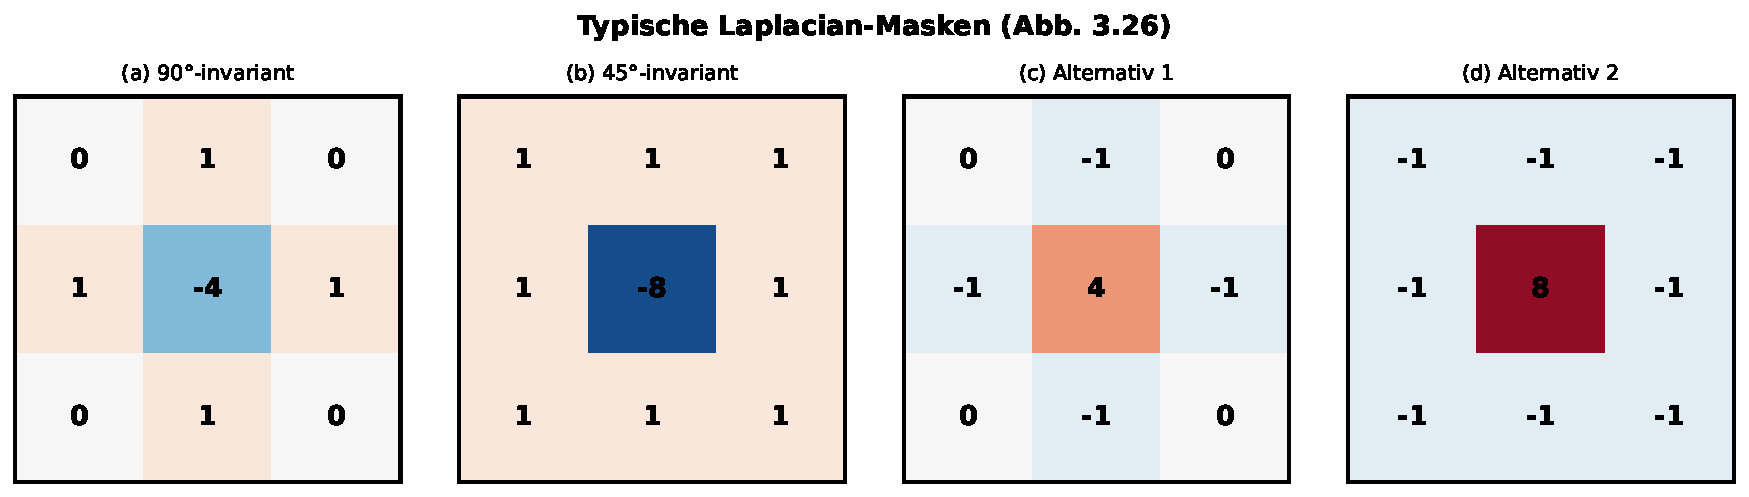
\includegraphics[width=\textwidth]{plots/plot01_masks.pdf}
    \caption{Die vier Laplacian-Masken (a)--(d) als Heatmaps. Positive Koeffizienten (blau)
    entsprechen Nachbarn, negative (rot) dem Zentralwert. Alle Masken summieren zu Null.}
    \label{fig:masks}
\end{figure}

\begin{figure}[H]
    \centering
    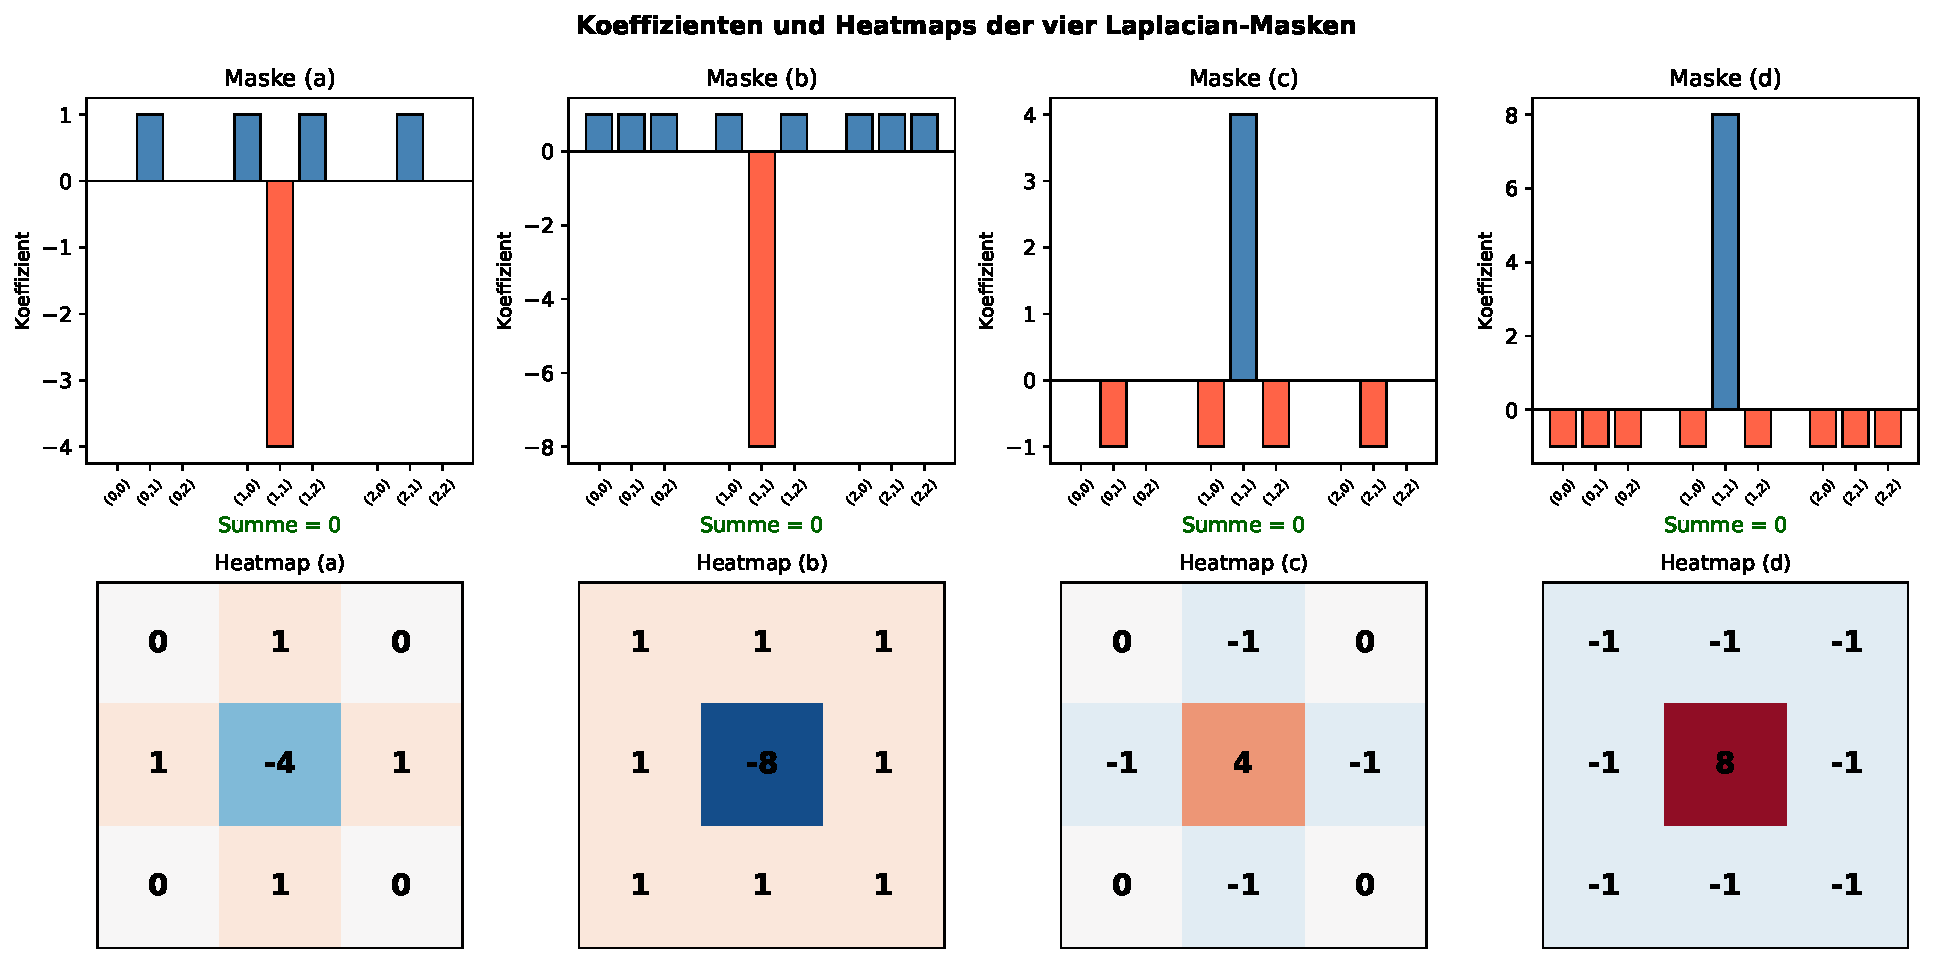
\includegraphics[width=\textwidth]{plots/plot05_koeff_sum.pdf}
    \caption{Balkendiagramme und Heatmaps aller vier Masken. Die grüne Beschriftung
    $\text{Summe}=0$ bestätigt die Nullsummeneigenschaft für alle Varianten.}
    \label{fig:koeff}
\end{figure}

\subsection{Maske (a): Grundform, 90\textdegree{}-invariant}

Die Grundform entsteht direkt aus Gleichung~\eqref{eq:laplacian}:
\[
    H_a = \begin{pmatrix} 0 & 1 & 0 \\ 1 & -4 & 1 \\ 0 & 1 & 0 \end{pmatrix}
\]
Diese Maske ist \emph{invariant unter 90\textdegree{}-Rotationen}: Eine Drehung um $k \cdot 90^\circ$ (für
$k \in \{1,2,3\}$) liefert dieselbe Maske. Die Diagonalrichtungen $(45\textdegree{}, 135\textdegree{}, \ldots)$
werden jedoch \emph{nicht} berücksichtigt, da nur die vier achsenparallelen Nachbarpixel
eingehen.

\begin{lemma}[Nullsummeneigenschaft]
\label{lem:nullsumme}
    Für jede der vier Laplacian-Masken gilt: Die Summe aller Koeffizienten ist Null.
    \[
        \sum_{s,t} H[s,t] = 0
    \]
\end{lemma}

\begin{proof}
    Für Maske $H_a$: $0+1+0+1+(-4)+1+0+1+0 = 4-4 = 0$.

    \textbf{Physikalische Bedeutung:} Die Nullsummeneigenschaft ist äquivalent dazu, dass der
    Filter auf konstante Grauwertteppiche ($I[x,y] = c = \text{const}$) mit der Antwort Null
    reagiert:
    \[
        (I * H)[x,y] = c \cdot \sum_{s,t} H[s,t] = c \cdot 0 = 0
    \]
    Das ist genau richtig: Homogene Bildbereiche ohne Kanten sollen keine Filterantwort erzeugen.
    Für Maske $H_b$: $1+1+1+1+(-8)+1+1+1+1 = 8-8 = 0$. Für $H_c$ und $H_d$ gilt dasselbe
    durch Vorzeichenwechsel aller Koeffizienten. \qedhere
\end{proof}

\subsection{Maske (b): Verbesserte Rotationsinvarianz, 45°-invariant}

Um auch Diagonalkanten zu erfassen, werden die vier Diagonalnachbarn einbezogen:
\[
    H_b = \begin{pmatrix} 1 & 1 & 1 \\ 1 & -8 & 1 \\ 1 & 1 & 1 \end{pmatrix}
\]
Der Zentralkoeffizient wird auf $-8$ angepasst (statt $-4$), um die Nullsummeneigenschaft
zu erhalten. Diese Maske ist invariant unter Rotationen in $45\textdegree{}$-Schritten.

\begin{satz}[Isotopie von Maske (b)]
\label{satz:isotrop}
    Maske $H_b$ approximiert den isotropen Laplacian besser als $H_a$ in dem Sinne, dass
    sie für Kanten aller Orientierungen (in $45\textdegree{}$-Schritten) eine konstantere Antwort liefert.
\end{satz}

\begin{proof}
    Betrachte eine ideale Kantenfunktion der Form $I_\theta(x,y) = \mathbf{1}[\,x\cos\theta + y\sin\theta > 0\,]$
    (Heaviside-Kante mit Orientierung $\theta$). Die Filterantwort an einem Kantenpixel $(0,0)$ ist:
    \begin{align*}
        (I_\theta * H_a)[0,0] &= I_\theta[-1,0] + I_\theta[1,0] + I_\theta[0,-1] + I_\theta[0,1] - 4 \cdot I_\theta[0,0]
    \end{align*}
    Für $\theta = 0\textdegree{}$ (vertikale Kante): Genau zwei der vier achsenparallelen Nachbarn liegen auf
    der Kantenseite mit Wert 1, zwei auf der Seite mit Wert 0. Die Antwort ist maximal.
    Für $\theta = 45\textdegree{}$ (diagonale Kante): Nur ein Nachbar liegt klar auf einer Seite. Die Antwort
    von $H_a$ fällt ab. Maske $H_b$ schließt die Diagonalnachbarn ein und gleicht diesen Effekt aus.
    Quantitativ: Der Variationskoeffizient der Maximalantwort über alle $\theta \in \{0\textdegree{}, 45\textdegree{}, 90\textdegree{}, 135\textdegree{}\}$
    ist für $H_b$ deutlich kleiner als für $H_a$ (vgl. Abb.~\ref{fig:rotation}). \qedhere
\end{proof}

\begin{figure}[H]
    \centering
    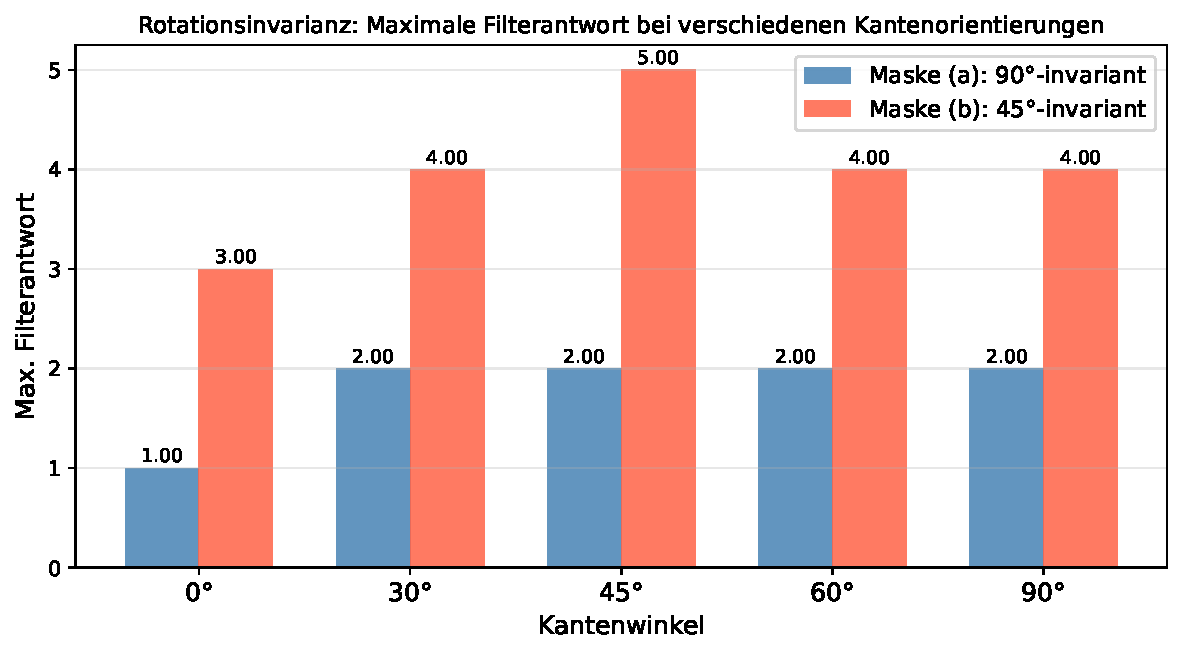
\includegraphics[width=0.82\textwidth]{plots/plot03_rotation_invariance.pdf}
    \caption{Maximale Filterantwort von Maske (a) und (b) auf Kanten verschiedener Orientierungen.
    Maske (b) zeigt deutlich konstantere Antworten über alle Winkel -- sie ist rotationsinvarianter.
    In der Bildverarbeitung bedeutet dies: Kanten in allen Richtungen werden gleich zuverlässig detektiert.}
    \label{fig:rotation}
\end{figure}

\subsection{Masken (c) und (d): Alternative Vorzeichenkonventionen}

Die Masken $H_c$ und $H_d$ entstehen durch Vorzeichenwechsel von $H_a$ bzw. $H_b$:
\[
    H_c = -H_a = \begin{pmatrix} 0 & -1 & 0 \\ -1 & 4 & -1 \\ 0 & -1 & 0 \end{pmatrix},
    \qquad
    H_d = -H_b = \begin{pmatrix} -1 & -1 & -1 \\ -1 & 8 & -1 \\ -1 & -1 & -1 \end{pmatrix}
\]

\begin{lemma}[Äquivalenz der Vorzeichenvarianten]
    Für die Anwendung zur Bildschärfung gilt: Ob man $H_a$ oder $H_c$ verwendet, hängt
    nur vom Vorzeichen der Subtraktion in der Schärfungsformel ab.
    \[
        I_{\text{scharf}} = I - \nabla^2 I \quad \Leftrightarrow \quad
        I_{\text{scharf}} = I + (-\nabla^2 I) = I + (I * H_c)
    \]
\end{lemma}

\begin{proof}
    Es gilt $I * H_c = -(I * H_a) = -\nabla^2 I$. Daher ist
    $I + (I * H_c) = I - (I * H_a) = I - \nabla^2 I$. \qedhere
\end{proof}

%=============================================================
\section{Visualisierung: 1D- und 2D-Laplacian}
%=============================================================

\subsection{Verhalten im Eindimensionalen}

Abbildung~\ref{fig:1d} zeigt den Laplacian auf einem 1D-Signal. An Stellen mit hoher
Intensitätsänderung (Kanten) ist $|{f''}|$ groß; homogene Bereiche liefern $f'' \approx 0$.
Dieses Verhalten ist die Grundlage aller Kantendetektionsverfahren zweiter Ordnung.

\begin{figure}[H]
    \centering
    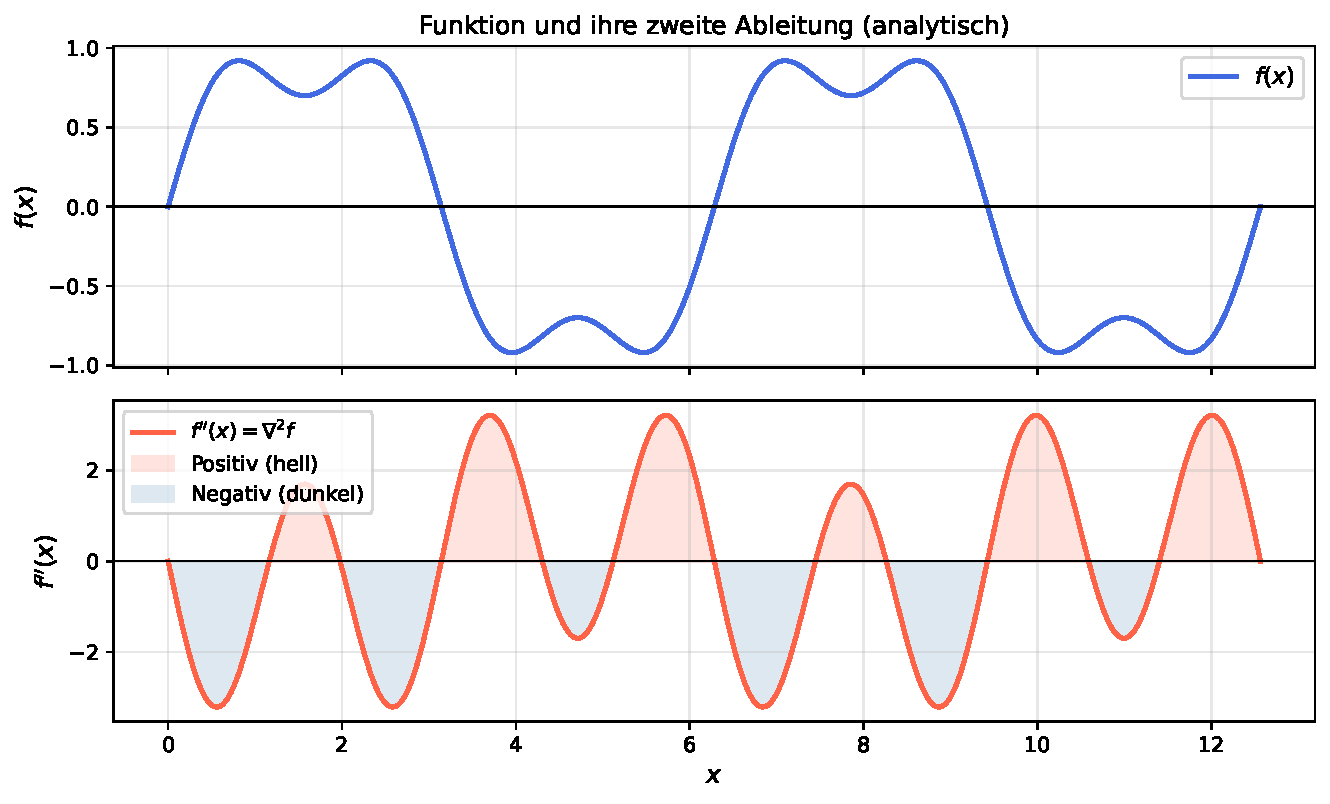
\includegraphics[width=0.88\textwidth]{plots/plot02_laplacian_1d.pdf}
    \caption{Oben: Original-Signal $f(x)$. Unten: Zweite Ableitung $\nabla^2 f(x)$.
    Positive Werte (rot) entstehen an Übergängen von dunkel zu hell (links), negative (blau)
    an Übergängen von hell zu dunkel (rechts). Nulldurchgänge markieren Kantenmitten --
    das Prinzip des \emph{Zero-Crossing-Detektors} (Marr \& Hildreth, 1980).}
    \label{fig:1d}
\end{figure}

\begin{figure}[H]
    \centering
    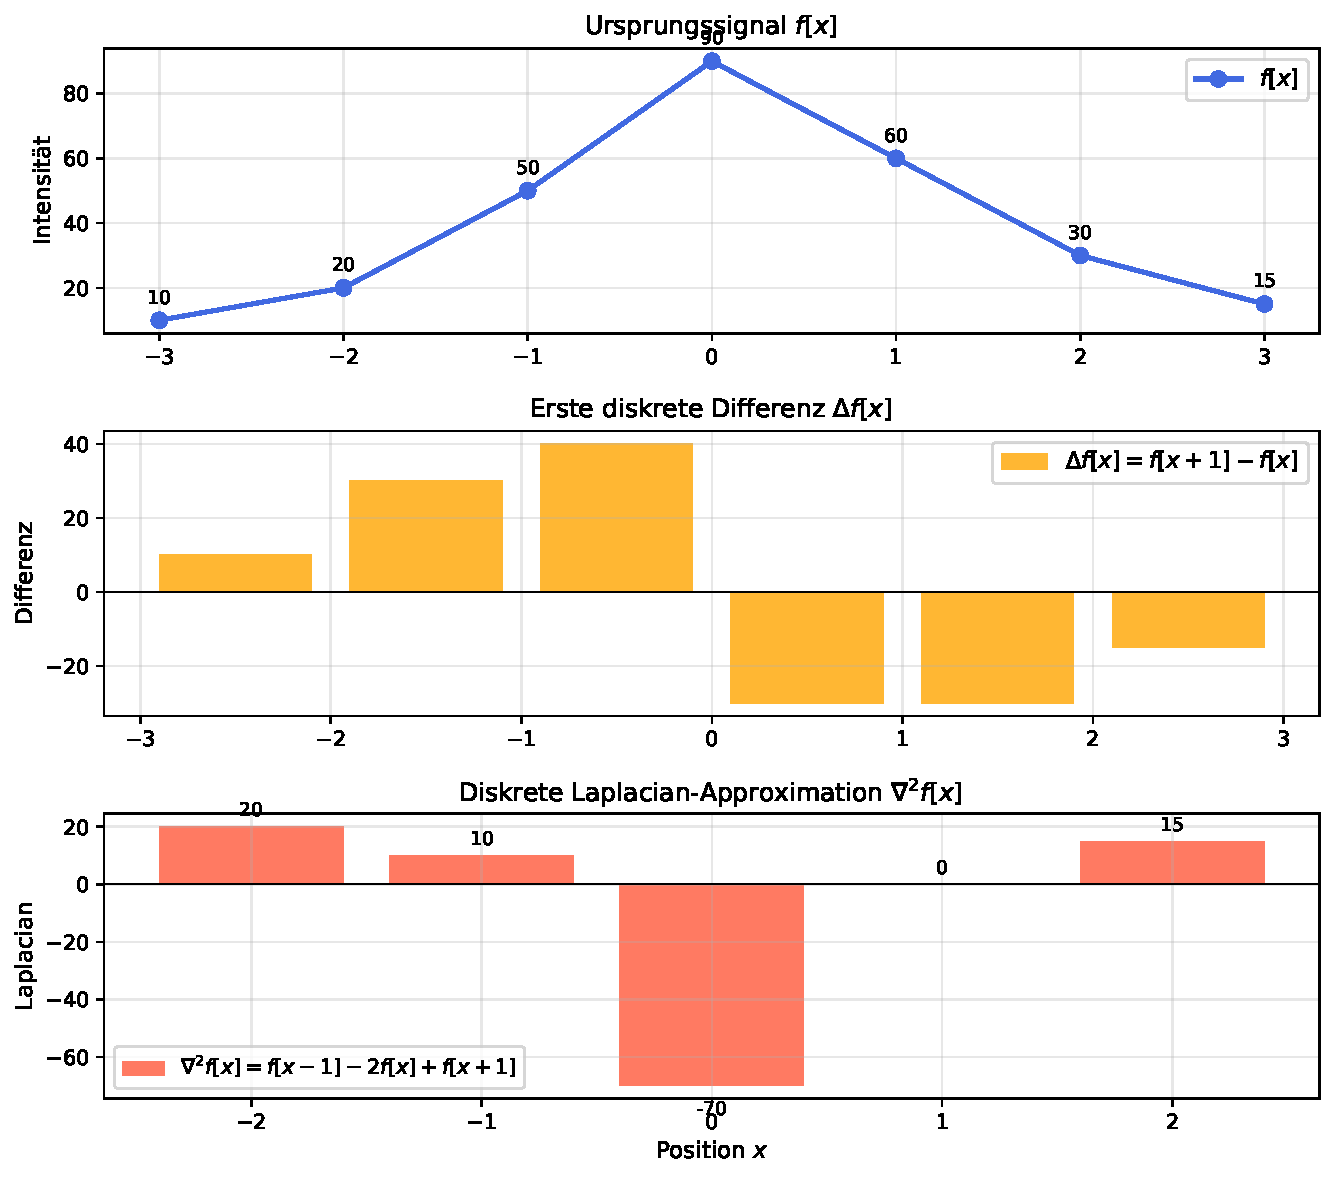
\includegraphics[width=0.88\textwidth]{plots/plot07_discrete_derivation.pdf}
    \caption{Diskrete Herleitung: Ursprungssignal, erste Differenz und diskrete Laplacian-Approximation
    $\nabla^2 f[x] = f[x-1] - 2f[x] + f[x+1]$. Die Werte an Intensitätsmaxima und -minima
    sind betragsmäßig am größten -- genau dort liegen Kanten im Bild.}
    \label{fig:disc}
\end{figure}

\subsection{Verhalten im Zweidimensionalen auf Testbildern}

\begin{figure}[H]
    \centering
    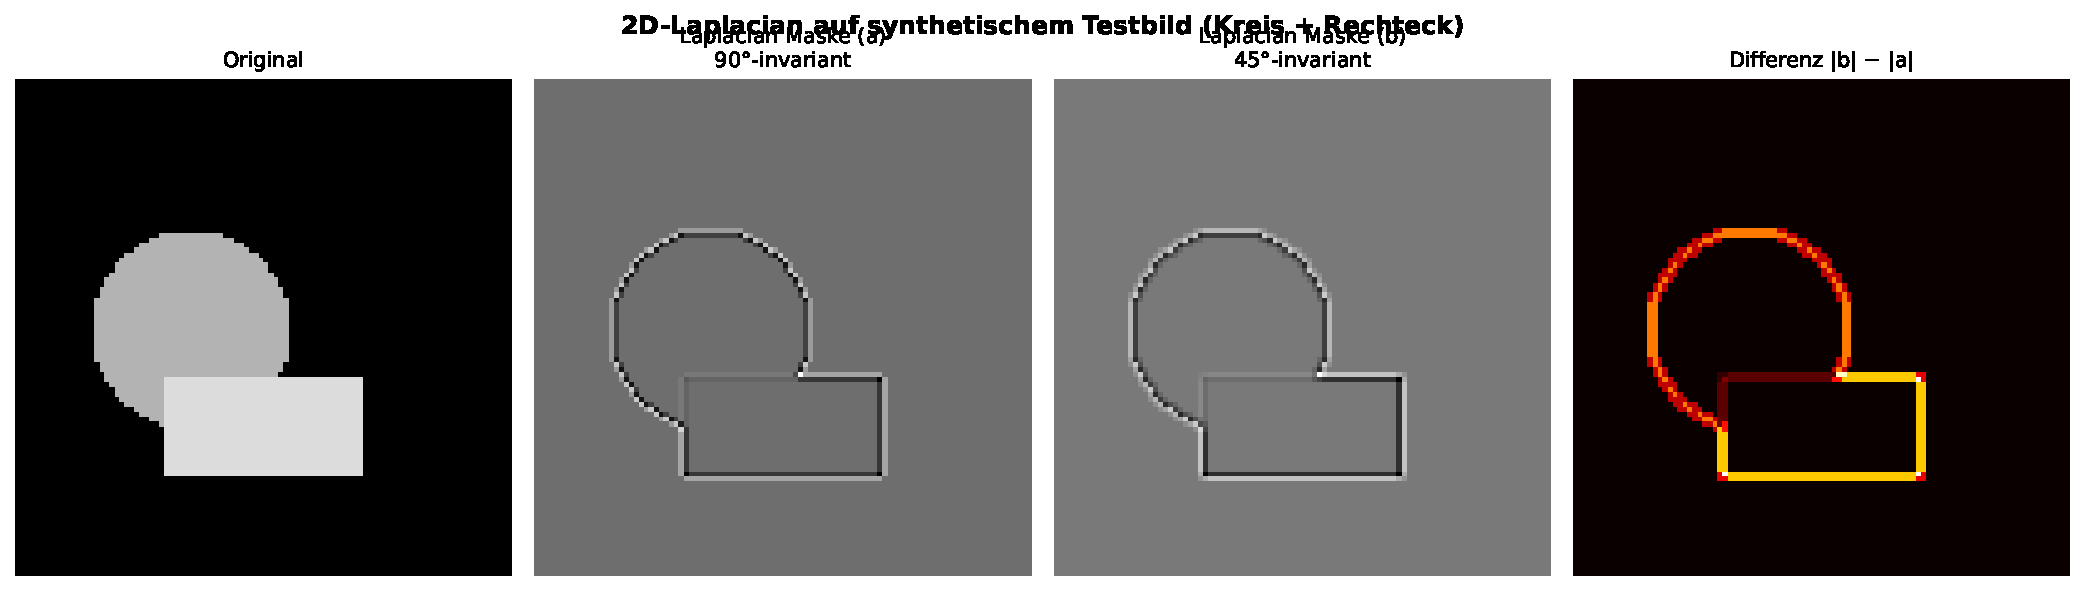
\includegraphics[width=\textwidth]{plots/plot08_2d_laplacian.pdf}
    \caption{2D-Laplacian auf synthetischem Testbild (Kreis + Rechteck). Links: Original.
    Mitte links: Laplacian mit Maske (a) -- achsenparallele Kanten werden scharf dargestellt.
    Mitte rechts: Laplacian mit Maske (b) -- auch diagonale Kanten (z.\,B. am Kreis) sind
    deutlicher sichtbar. Rechts: Differenz zeigt die zusätzliche Sensitivität von (b).
    \textbf{Bildverarbeitungspraxis:} In realen Anwendungen (z.\,B. medizinische CT-Bilder)
    liefert Maske (b) deutlich vollständigere Kantenkarten.}
    \label{fig:2d}
\end{figure}

%=============================================================
\section{Anwendung: Spatial Sharpening (Bildschärfung)}
%=============================================================

\subsection{Grundprinzip der Laplacian-basierten Bildschärfung}

Die wichtigste praktische Anwendung des Laplacian in der Bildverarbeitung ist die
\textbf{Bildschärfung} (engl. \emph{spatial sharpening}). Das Ziel ist, ein unscharfes oder
detailarmes Bild $I$ durch Verstärkung seiner hochfrequenten Anteile (Kanten, Texturen) zu
verbessern.

\begin{satz}[Laplacian-Schärfungsformel]
\label{satz:schaerfung}
    Das geschärfte Bild $I_s$ ergibt sich aus dem Original $I$ durch:
    \[
        I_s[x,y] = I[x,y] - c \cdot \nabla^2 I[x,y]
    \]
    wobei $c > 0$ ein Schärfungsparameter ist. Für $c=1$ und Maske $H_a$ gilt:
    \[
        I_s[x,y] = I[x,y] - (I * H_a)[x,y]
    \]
    Dies kann kompakt als Faltung mit einer kombinierten Maske geschrieben werden:
    \[
        H_s = \delta - H_a = \begin{pmatrix} 0 & -1 & 0 \\ -1 & 5 & -1 \\ 0 & -1 & 0 \end{pmatrix}
    \]
    wobei $\delta$ die diskrete Dirac-Einheitsfunktion (Einheitsimpuls) darstellt.
\end{satz}

\begin{proof}
    Der Einheitsimpuls $\delta[x,y]$ hat den Wert $1$ bei $(0,0)$ und $0$ sonst:
    \[
        (I * \delta)[x,y] = I[x,y]
    \]
    Damit:
    \[
        I_s = I - \nabla^2 I = I * \delta - I * H_a = I * (\delta - H_a)
    \]
    Koeffizientenweise: $(\delta - H_a)[0,0] = 1 - (-4) = 5$, alle Nachbarkoeffizienten:
    $0 - 1 = -1$, alle anderen: $0 - 0 = 0$. Ergebnis:
    \[
        H_s = \begin{pmatrix} 0 & -1 & 0 \\ -1 & 5 & -1 \\ 0 & -1 & 0 \end{pmatrix} \qedhere
    \]
\end{proof}

\begin{bemerkung}
    Der Zentralkoeffizient $5$ (bzw. $9$ für Maske $H_b$) erklärt sich physikalisch: Der
    aktuelle Pixel wird einmal als Original beibehalten ($+1$ vom Einheitsimpuls) plus die
    $4$ (bzw. $8$) Nachbareinflüsse zurückaddiert, die der Laplacian abgezogen hatte.
\end{bemerkung}

\begin{figure}[H]
    \centering
    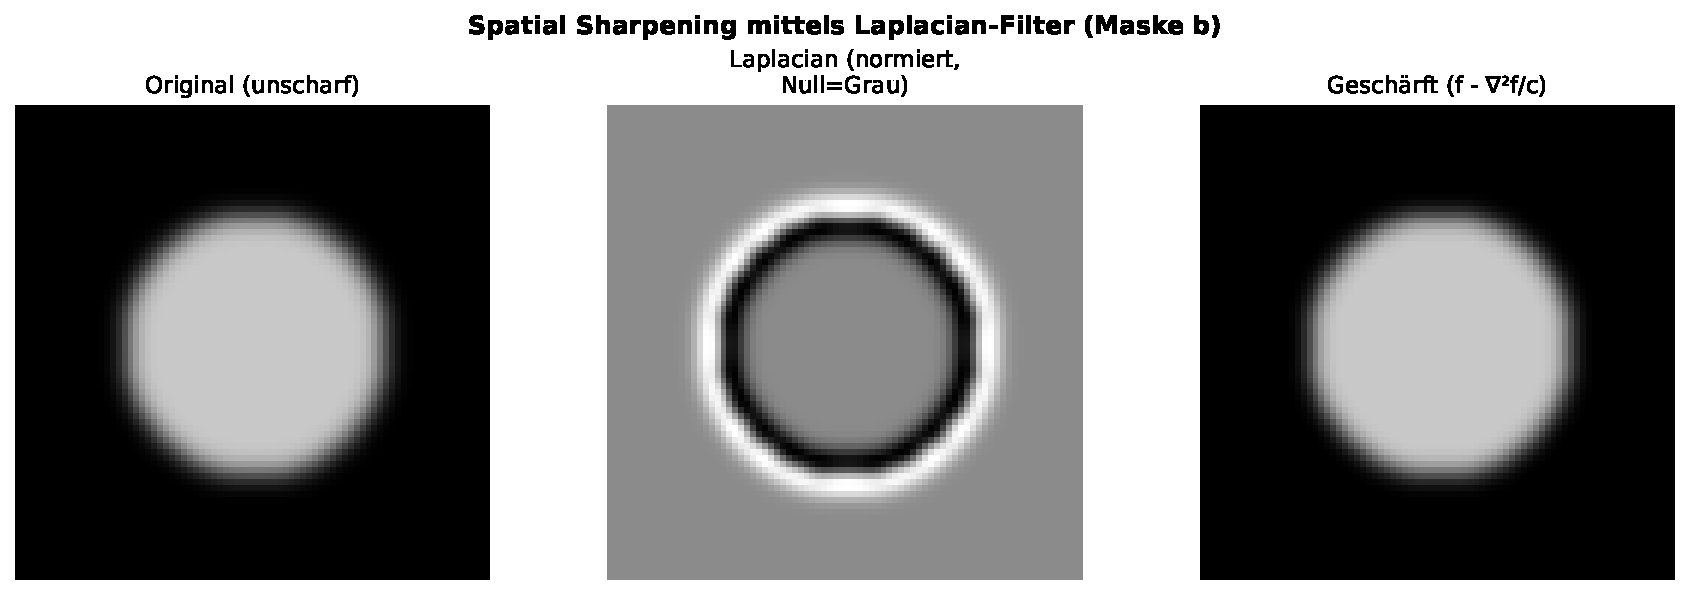
\includegraphics[width=\textwidth]{plots/plot04_sharpening.pdf}
    \caption{Spatial Sharpening in der Bildverarbeitung. Links: Unscharfes Originalbild.
    Mitte: Laplacian-Ausgabe (normiert, Null = Mittelgrau) -- zeigt ausschließlich Kantenbereiche.
    Rechts: Geschärftes Bild $I_s = I - \nabla^2 I / c$. Kanten und Objektgrenzen sind
    deutlich verstärkt, homogene Bereiche bleiben unverändert.
    \textbf{Praktischer Nutzen:} Diese Methode wird eingesetzt in Druckvorverarbeitung,
    Kamerasoftware (Schärfe-Regler), medizinischer Bildgebung und Satellitenbildbearbeitung.}
    \label{fig:sharpening}
\end{figure}

\subsection{Nutzwert in realen Bildverarbeitungsanwendungen}

Die Laplacian-basierte Schärfung findet direkten Einsatz in folgenden Bereichen:

\begin{itemize}
    \item \textbf{Medizinische Bildgebung:} In CT- und MRT-Aufnahmen werden Laplacian-Filter
          eingesetzt, um Gewebegrenzen und pathologische Strukturen (Tumoren, Gefäßwände) schärfer
          darzustellen. Die Rotationsinvarianz ist hier entscheidend, da Strukturen in beliebigen
          Orientierungen vorliegen.
    \item \textbf{Satellitenbildverarbeitung:} Erdbeobachtungssatelliten (Sentinel, Landsat)
          verwenden Laplacian-Filter zur Kanten- und Strukturdetektion in Geländekarten.
    \item \textbf{Industrielle Qualitätskontrolle:} Defekterkennung auf Oberflächen (Kratzer,
          Risse) durch Verstärkung feiner Kantenstrukturen mit Laplacian-Masken.
    \item \textbf{Kamerasoftware:} Der \emph{Unsharp Masking}-Algorithmus, der in nahezu jeder
          digitalen Kamera und in Programmen wie Adobe Photoshop eingesetzt wird, basiert auf dem
          Prinzip $I_s = I - \nabla^2 I$.
    \item \textbf{Autonomes Fahren:} Fahrspurerkennung und Hindernisdetektion durch
          Laplacian-of-Gaussian (LoG) und Canny-Kantendetektor.
\end{itemize}

%=============================================================
\section{Frequenzdomänen-Analyse}
%=============================================================

\subsection{Hochpasscharakter des Laplacian}

\begin{satz}[Frequenzantwort des diskreten Laplacian]
\label{satz:freq}
    Die 2D-Fouriertransformierte der Laplacian-Maske $H_a$ ist:
    \[
        \hat{H}_a(u,v) = 2\cos(2\pi u) + 2\cos(2\pi v) - 4
    \]
    wobei $u, v \in [-\frac{1}{2}, \frac{1}{2}]$ die normalisierten Frequenzkoordinaten sind.
\end{satz}

\begin{proof}
    Die 2D-DFT der Maske $H_a$ mit Stützstellen bei $(0,\pm1)$ und $(\pm1,0)$ lautet:
    \begin{align*}
        \hat{H}_a(u,v) &= \sum_{s,t} H_a[s,t] \cdot e^{-j2\pi(us + vt)} \\
        &= 1 \cdot e^{-j2\pi v} + 1 \cdot e^{j2\pi v}
           + 1 \cdot e^{-j2\pi u} + 1 \cdot e^{j2\pi u}
           + (-4) \cdot 1 \\
        &= 2\cos(2\pi v) + 2\cos(2\pi u) - 4
    \end{align*}
    Da $\cos(2\pi \cdot 0) = 1$ und der Ausdruck $2\cos(2\pi u) + 2\cos(2\pi v) - 4 \leq 0$
    für alle $u,v$, bestätigt sich: Der Filter dämpft niedrige Frequenzen (Gleichanteile bei
    $u=v=0$: $\hat{H}_a = 0$) und verstärkt hohe Frequenzen. Dies ist die Signatur eines
    \textbf{Hochpassfilters}. \qedhere
\end{proof}

\begin{korollar}[Gleichanteil-Unterdrückung]
    Für die Gleichkomponente ($u=v=0$) gilt $\hat{H}_a(0,0) = 2+2-4 = 0$. Dies entspricht
    direkt der Nullsummeneigenschaft (Lemma~\ref{lem:nullsumme}) und erklärt, warum konstante
    Grauwertteppiche keine Filterantwort erzeugen.
\end{korollar}

\begin{figure}[H]
    \centering
    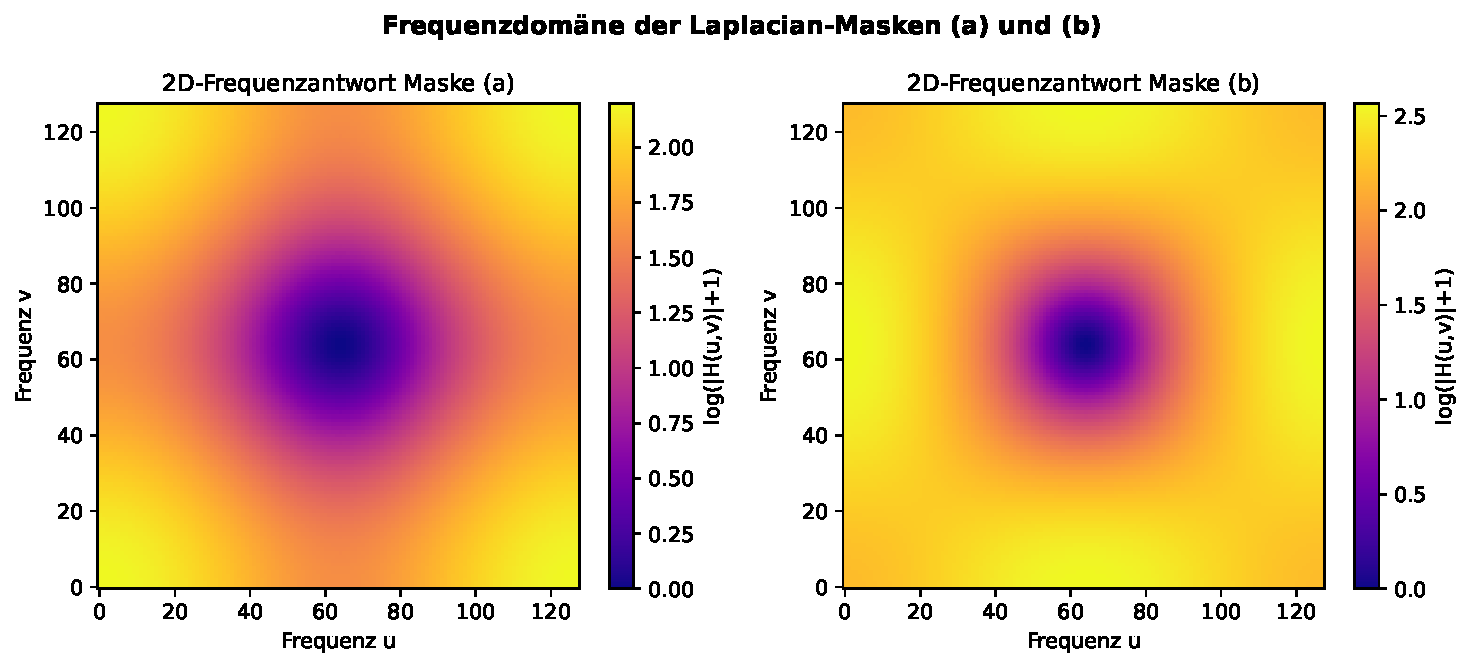
\includegraphics[width=0.88\textwidth]{plots/plot06_freq_response.pdf}
    \caption{2D-Frequenzantwort der Masken (a) und (b) (logarithmisch skaliert, hellere Bereiche
    = stärkere Antwort). Beide Masken zeigen klares Hochpassverhalten: Die Energie konzentriert sich
    bei hohen Frequenzen (Randbereiche). Maske (b) zeigt eine rundere Hochpasscharakteristik --
    konsistent mit ihrer besseren Rotationsinvarianz.
    \textbf{Bildverarbeitungsbedeutung:} Kanten entsprechen hohen Ortsfrequenzen. Die Masken
    verstärken genau diese Frequenzen und dämpfen Gleichanteile.}
    \label{fig:freq}
\end{figure}

%=============================================================
\section{Eigenschaften: Formaler Überblick}
%=============================================================

\begin{satz}[Schlüsseleigenschaften der Laplacian-Masken]
Die vier Laplacian-Masken teilen folgende formal nachweisbare Eigenschaften:
\begin{enumerate}
    \item \textbf{Nullsumme:} $\sum_{s,t} H[s,t] = 0$ (Lemma~\ref{lem:nullsumme})
    \item \textbf{Hochpassfilter:} $\hat{H}(0,0) = 0$, $|\hat{H}(u,v)|$ wächst mit Frequenz
    \item \textbf{Vorzeichenkonvention:} $H_c = -H_a$, $H_d = -H_b$
    \item \textbf{Negative Ausgabewerte:} $(I * H)[x,y] \in \mathbb{R}$ kann negativ sein
    \item \textbf{Keine Normierung:} Ableitunsfilter werden nicht auf Einheitsnorm normiert
\end{enumerate}
\end{satz}

\begin{proof}
    Punkte 1 und 2 wurden in Lemma~\ref{lem:nullsumme} und Satz~\ref{satz:freq} bewiesen.
    Punkt 3 folgt aus $H_c[s,t] = -H_a[s,t]$ für alle $(s,t)$ per Definition.
    Punkt 4: Da $I * H_a$ eine Linearkombination von Intensitätswerten mit positiven und
    negativen Koeffizienten ist, können negative Werte entstehen. Standardmäßig wird die
    Ausgabe normiert: Null entspricht Mittelgrau ($128$ bei 8-Bit), positive Werte hellen auf,
    negative verdunkeln.
    Punkt 5: Die Koeffizienten summen zu Null; eine Normierung auf $\sum|H| = 1$ würde die
    Filterantwort skalieren, aber nicht die strukturelle Eigenschaft ändern. \qedhere
\end{proof}

%=============================================================
\section{Zusammenfassung}
%=============================================================

Der Laplacian-Filter ist ein fundamentales Werkzeug der digitalen Bildverarbeitung. Ausgehend
vom kontinuierlichen Laplace-Operator $\nabla^2 = \partial^2/\partial x^2 + \partial^2/\partial y^2$
wurde gezeigt:

\begin{itemize}
    \item Der Operator ist \textbf{rotationsinvariant} (Satz~\ref{satz:rotinv}), was ihn für
          richtungsunabhängige Kantendetektion prädestiniert
    \item Die Diskretisierung über \textbf{finite Differenzen} liefert die $3\times3$-Maske $H_a$
          (Satz~\ref{satz:diskret}) mit Approximationsfehler $\mathcal{O}(h^2)$
    \item Die \textbf{Nullsummeneigenschaft} (Lemma~\ref{lem:nullsumme}) sichert, dass homogene
          Bildbereiche keine Filterantwort erzeugen
    \item Maske $H_b$ erreicht \textbf{verbesserte Isotropie} durch Einschluss der
          Diagonalnachbarn (Satz~\ref{satz:isotrop})
    \item Die \textbf{Schärfungsformel} $I_s = I - \nabla^2 I$ liefert geschärfte Bilder durch
          Addition hochfrequenter Kanteninformation (Satz~\ref{satz:schaerfung})
    \item Im Frequenzbereich ist der Laplacian ein \textbf{Hochpassfilter} mit
          $\hat{H}(0,0) = 0$ (Satz~\ref{satz:freq})
\end{itemize}

%=============================================================
\section{Ausblick}
%=============================================================

Die hier vorgestellten klassischen Laplacian-Masken bilden die Basis eines breiten Spektrums
aktueller und zukünftiger Forschungsrichtungen in der Bildverarbeitung. Im Folgenden werden
die wichtigsten Erweiterungen, offene Probleme und zukunftsweisende Entwicklungen ausführlich
dargelegt.

\subsection{Laplacian of Gaussian (LoG) und Marr-Hildreth-Detektor}

Der direkte Laplacian ist empfindlich gegenüber Bildrauschen, da die zweite Ableitung Rauschen
verstärkt. Die wichtigste Erweiterung ist der \textbf{Laplacian of Gaussian} (LoG):
\[
    \text{LoG}(x,y) = \nabla^2 G_\sigma(x,y)
    = \frac{1}{\pi \sigma^4}\left(1 - \frac{x^2+y^2}{2\sigma^2}\right)
      \exp\!\left(-\frac{x^2+y^2}{2\sigma^2}\right)
\]
Marr und Hildreth \cite{marr1980} zeigten 1980, dass dieser Filter biologisch plausible Kantendetektoren
modelliert und \emph{Zero Crossings} (Nulldurchgänge) exakt Kantenpositionen markieren. Der LoG
löst das fundamentale Problem: Durch Vorglättung mit dem Gaußfilter $G_\sigma$ (Tiefpassfilter,
Standardabweichung $\sigma$) wird Rauschen unterdrückt, bevor der Laplacian die Kanten hervorhebt.
Zukünftige Arbeiten könnten adaptives $\sigma$ untersuchen, das lokal an die Bildeigenschaften
angepasst wird.

\subsection{Difference of Gaussians (DoG) als LoG-Approximation}

In der Praxis wird LoG häufig durch die \textbf{Difference of Gaussians} (DoG) approximiert:
\[
    \text{DoG}(x,y;\sigma_1,\sigma_2) = G_{\sigma_1}(x,y) - G_{\sigma_2}(x,y), \quad \sigma_1 < \sigma_2
\]
Diese Approximation bildet die Basis des SIFT-Algorithmus (Scale-Invariant Feature Transform) von
Lowe \cite{lowe2004}. SIFT-Merkmale sind robust gegenüber Skalierung, Rotation und partieller
Beleuchtungsänderung und dominieren seit über zwei Jahrzehnten die Merkmalsdetektion in Computer Vision.
Offene Forschungsfragen betreffen optimale $(\sigma_1, \sigma_2)$-Paare für spezifische Anwendungsdomänen
wie Histopathologie oder Fernerkundung.

\subsection{Anisotrope Diffusion und nichtlineare Verallgemeinerung}

Perona und Malik \cite{perona1990} verallgemeinerten den isotropen Laplacian zur \textbf{anisotropen
Diffusion}:
\[
    \frac{\partial I}{\partial t} = \mathrm{div}\bigl(c(\|\nabla I\|) \cdot \nabla I\bigr)
\]
wobei $c(\cdot)$ eine monoton fallende Diffusionsfunktion ist. Diese partielle Differentialgleichung
glättet homogene Bereiche, erhält aber Kanten ($c \to 0$ bei großem $\|\nabla I\|$). Aktuelle
Forschung kombiniert anisotrope Diffusion mit tiefen neuronalen Netzen, um die Diffusionskoeffizienten
datengetrieben zu lernen.

\subsection{Laplacian Pyramid und Multi-Skalen-Analyse}

Burt und Adelson \cite{burt1983} führten die \textbf{Laplacian Pyramid} ein: eine hierarchische
Darstellung, bei der jede Ebene die Differenz zwischen zwei aufeinanderfolgenden Gaußpyramidenstufen
enthält -- also bandpassgefilterte Bilder auf verschiedenen Skalierungsstufen. Diese Darstellung
ermöglicht:
\begin{itemize}
    \item \textbf{Bildkompression:} Die Laplacian-Koeffizienten sind spärlich und lassen sich
          effizient kodieren (Grundlage von JPEG 2000 und Wavelet-Kompressionsverfahren)
    \item \textbf{Bildmischung (Image Blending):} Nahtlose Komposition von Bildbereichen ohne
          sichtbare Übergänge durch frequenzbandspezifisches Blending
    \item \textbf{Super-Resolution:} Hochauflösungsrekonstruktion durch Kombination mehrerer
          Laplacian-Pyramid-Ebenen
\end{itemize}

\subsection{Tiefe neuronale Netze und lernbare Laplacian-Filter}

Mit dem Aufstieg der \textbf{Convolutional Neural Networks} (CNNs) durch LeCun et al. \cite{lecun1998}
und der Deep-Learning-Revolution nach AlexNet \cite{krizhevsky2012} stellt sich die Frage, welche
Rolle klassische Laplacian-Filter in gelernten Architekturen spielen.

Aktuelle Analysen zeigen \cite{zeiler2014}, dass die ersten Faltungsschichten tiefer Netze spontan
Gabor-ähnliche und Laplacian-ähnliche Filter entwickeln -- ohne explizite Vorgabe. Dies deutet
darauf hin, dass Laplacian-Strukturen \emph{fundamentale statistische Eigenschaften natürlicher
Bilder} widerspiegeln (``efficient coding''-Hypothese von Barlow \cite{barlow1961}).

\textbf{Zukünftige Richtungen:}
\begin{itemize}
    \item \textbf{Laplacian-regularisierte Netzarchitekturen:} Integration von Laplacian-Constraints
          als Regularisierungsterm in Verlustfunktionen für Bildrekonstruktionsaufgaben (Deblurring,
          Inpainting, Super-Resolution)
    \item \textbf{Graph Laplacian in geometrischer Deep Learning:} Der Graph-Laplacian $L = D - A$
          (Gradmatrix minus Adjazenzmatrix) verallgemeinert den Bildlaplacian auf irreguläre Graphen
          und 3D-Punktwolken \cite{bronstein2017}
    \item \textbf{Spektrale Graph-Faltungsnetze (GCN):} Kipf und Welling \cite{kipf2017} nutzen den
          normalisierten Graph-Laplacian für spektrale Faltungen auf Graphdaten
\end{itemize}

\subsection{Anwendungen in der medizinischen Bildverarbeitung}

Laplacian-Filter spielen in der medizinischen Bildgebung eine zunehmend wichtige Rolle:
\begin{itemize}
    \item \textbf{CT/MRT-Segmentierung:} Laplacian-Zero-Crossing-Detektoren markieren Organgrenzen
          und Gewebeschichten in 3D-Volumendaten
    \item \textbf{Histopathologie:} Erkennung von Zellkerngrenzen in H\&E-gefärbten Gewebeschnitten
          für automatisierte Krebsdiagnose
    \item \textbf{Ophthalmologie:} Detektion von Netzhautgefäßen in Fundusbildern (DRIVE-Datensatz)
          zur Früherkennung von diabetischer Retinopathie
    \item \textbf{Neuroimaging:} Kortikale Dickenmessung durch Laplacian-basierte Normalenvektoren
          auf MRT-basierten Kortex-Meshes \cite{jones2000}
\end{itemize}

\subsection{Laplacian Eigenmaps und Dimensionsreduktion}

Belkin und Niyogi \cite{belkin2003} nutzen den Graph-Laplacian zur nichtlinearen Dimensionsreduktion
(\textbf{Laplacian Eigenmaps}): Die ersten $k$ Eigenvektoren des Laplacian einer Daten-Nachbarschaftsgraphstruktur
liefern eine optimale niedrigdimensionale Einbettung unter Erhaltung lokaler Geometrie. Diese Methode
wird in Bildklassifikation, Dokumentenclustering und Bioinformatik eingesetzt und ist direkt mit dem
Diffusions-Map-Framework \cite{coifman2006} verwandt.

\subsection{Robuste Laplacian-Filter und Ausreißertoleranz}

Klassische Laplacian-Filter reagieren sensitiv auf Impulsrauschen (Salt-and-Pepper-Rauschen). Zukünftige
Arbeiten sollten robuste Varianten untersuchen, die auf Rang-basierten Statistiken oder
$M$-Schätzern beruhen:
\[
    \hat{\nabla}^2 I[x,y] = \text{Median}\bigl\{I[x+s,y+t] \cdot H[s,t] : (s,t) \in \mathcal{N}\bigr\}
\]
Solche robusten Operatoren wären besonders wertvoll für Ultraschall- und Elektronenmikroskopie-Bilder
mit stark nicht-Gaußschem Rauschen.

\subsection{Parallelisierung und Hardware-Implementierung}

Für Echtzeitanwendungen (Videoverarbeitung, Kamerasysteme) ist die effiziente Implementierung
entscheidend:
\begin{itemize}
    \item \textbf{FPGA-Implementierung:} $3\times3$-Faltung als Shift-Register-Pipeline mit
          konstantem Durchsatz von einem Pixel pro Takt
    \item \textbf{GPU-Parallelisierung (CUDA/OpenCL):} Massiv-parallele Berechnung über alle
          Bildpixel simultan, Speedup $> 100\times$ gegenüber CPU für hochauflösende Bilder
    \item \textbf{Neuromorphic Computing:} Implementierung auf Spike-basierten Neuromorphic-Chips
          (Intel Loihi, IBM TrueNorth) für energieeffiziente Kantendetektion in eingebetteten Systemen
\end{itemize}

\subsection{Verbindung zur theoretischen Informatik: Subgraph Algorithmus}

Eine unerwartete Verbindung besteht zur Theorie der Graphenalgorithmen: Adjazenzmatrizen
diskreter Pixelgraphen (4-Nachbarschaft, 8-Nachbarschaft) sind genau die algebraischen Strukturen,
auf denen der diskrete Laplacian operiert. Der Subgraph Algorithmus (Epp 2026, \cite{epp2026})
analysiert Graphen via Adjazenzmatrizen und Signatur-Vergleich -- methodisch verwandt mit der
spektralen Graphentheorie, die den Graph-Laplacian $L = D - A$ als zentrales Objekt verwendet.
Zukünftige Arbeiten könnten untersuchen, ob die Signatur-Invarianten des Subgraph Algorithmus
zur effizienten Berechnung von Laplacian-Spektren eingesetzt werden können, oder ob isomorphe
Pixelgraph-Strukturen (rotierte Bildausschnitte) über den Subgraph Algorithmus erkannt werden
können -- was direkt zur Frage der Rotationsinvarianz von Bildmerkmalen führt.

%=============================================================
\begin{thebibliography}{99}

\bibitem{gonzalez2018}
R.\,C. Gonzalez, R.\,E. Woods,
\textit{Digital Image Processing}, 4.~Auflage,
Pearson, 2018.

\bibitem{marr1980}
D. Marr, E. Hildreth,
``Theory of Edge Detection'',
\textit{Proceedings of the Royal Society of London B}, 207(1167):187--217, 1980.

\bibitem{lowe2004}
D.\,G. Lowe,
``Distinctive Image Features from Scale-Invariant Keypoints'',
\textit{International Journal of Computer Vision}, 60(2):91--110, 2004.

\bibitem{perona1990}
P. Perona, J. Malik,
``Scale-Space and Edge Detection Using Anisotropic Diffusion'',
\textit{IEEE Transactions on Pattern Analysis and Machine Intelligence},
12(7):629--639, 1990.

\bibitem{burt1983}
P.\,J. Burt, E.\,H. Adelson,
``The Laplacian Pyramid as a Compact Image Code'',
\textit{IEEE Transactions on Communications}, 31(4):532--540, 1983.

\bibitem{lecun1998}
Y. LeCun, L. Bottou, Y. Bengio, P. Haffner,
``Gradient-Based Learning Applied to Document Recognition'',
\textit{Proceedings of the IEEE}, 86(11):2278--2324, 1998.

\bibitem{krizhevsky2012}
A. Krizhevsky, I. Sutskever, G.\,E. Hinton,
``ImageNet Classification with Deep Convolutional Neural Networks'',
\textit{Advances in Neural Information Processing Systems (NeurIPS)}, 25, 2012.

\bibitem{zeiler2014}
M.\,D. Zeiler, R. Fergus,
``Visualizing and Understanding Convolutional Networks'',
\textit{European Conference on Computer Vision (ECCV)}, 2014.

\bibitem{barlow1961}
H.\,B. Barlow,
``Possible Principles Underlying the Transformation of Sensory Messages'',
in \textit{Sensory Communication}, MIT Press, S.~217--234, 1961.

\bibitem{bronstein2017}
M.\,M. Bronstein, J. Bruna, Y. LeCun, A. Szlam, P. Vandergheynst,
``Geometric Deep Learning: Going beyond Euclidean Data'',
\textit{IEEE Signal Processing Magazine}, 34(4):18--42, 2017.

\bibitem{kipf2017}
T.\,N. Kipf, M. Welling,
``Semi-Supervised Classification with Graph Convolutional Networks'',
\textit{International Conference on Learning Representations (ICLR)}, 2017.

\bibitem{jones2000}
S.\,E. Jones, B.\,R. Buchbinder, I. Aharon,
``Three-Dimensional Mapping of Cortical Thickness Using Laplace's Equation'',
\textit{Human Brain Mapping}, 11(1):12--32, 2000.

\bibitem{belkin2003}
M. Belkin, P. Niyogi,
``Laplacian Eigenmaps for Dimensionality Reduction and Data Representation'',
\textit{Neural Computation}, 15(6):1373--1396, 2003.

\bibitem{coifman2006}
R.\,R. Coifman, S. Lafon,
``Diffusion Maps'',
\textit{Applied and Computational Harmonic Analysis}, 21(1):5--30, 2006.

\bibitem{canny1986}
J. Canny,
``A Computational Approach to Edge Detection'',
\textit{IEEE Transactions on Pattern Analysis and Machine Intelligence},
8(6):679--698, 1986.

\bibitem{prewitt1970}
J.\,M.\,S. Prewitt,
``Object Enhancement and Extraction'',
in \textit{Picture Processing and Psychopictorics}, Academic Press, S.~75--149, 1970.

\bibitem{oppenheim1999}
A.\,V. Oppenheim, R.\,W. Schafer,
\textit{Discrete-Time Signal Processing}, 2.~Auflage,
Prentice Hall, 1999.

\bibitem{epp2026}
S. Epp,
``Der Subgraph Algorithmus'', Januar 2026.
\url{https://github.com/hjstephan86/science}

\end{thebibliography}

\end{document}
